\documentclass[a4paper, 11pt]{article}
\usepackage{comment} % enables the use of multi-line comments (\ifx \fi) 
\usepackage{fullpage} % changes the margin
\usepackage{amsmath}
\usepackage[makeroom]{cancel}

\usepackage{graphicx}
\usepackage[]{textcomp}

\usepackage{tikz}
\usetikzlibrary{arrows,automata}

\usepackage{fixltx2e}

\usepackage{geometry}
 \geometry{
 a4paper,
 left=15mm,
 right=15mm,
 top=15mm,
 }

\begin{document}

\noindent 
\includegraphics[scale=0.2]{figures/logo.png}\\
\large \textbf{Systèmes Logiques - EE-102}\hfill \textbf{Valentin RIAT, Rafael RIBER}\\
 \hfill \large \textbf{Projet de semestre: Réveil-matin de voyage}\hfill \textbf{EL-BA2 - 2018-2019}

\section{Déscription générale et mode d'emploi}
UNE PAGE

\section{Solutions techniques}
DEUX PAGES

\subsection{Machine d'états finis générale}
\begin{center}
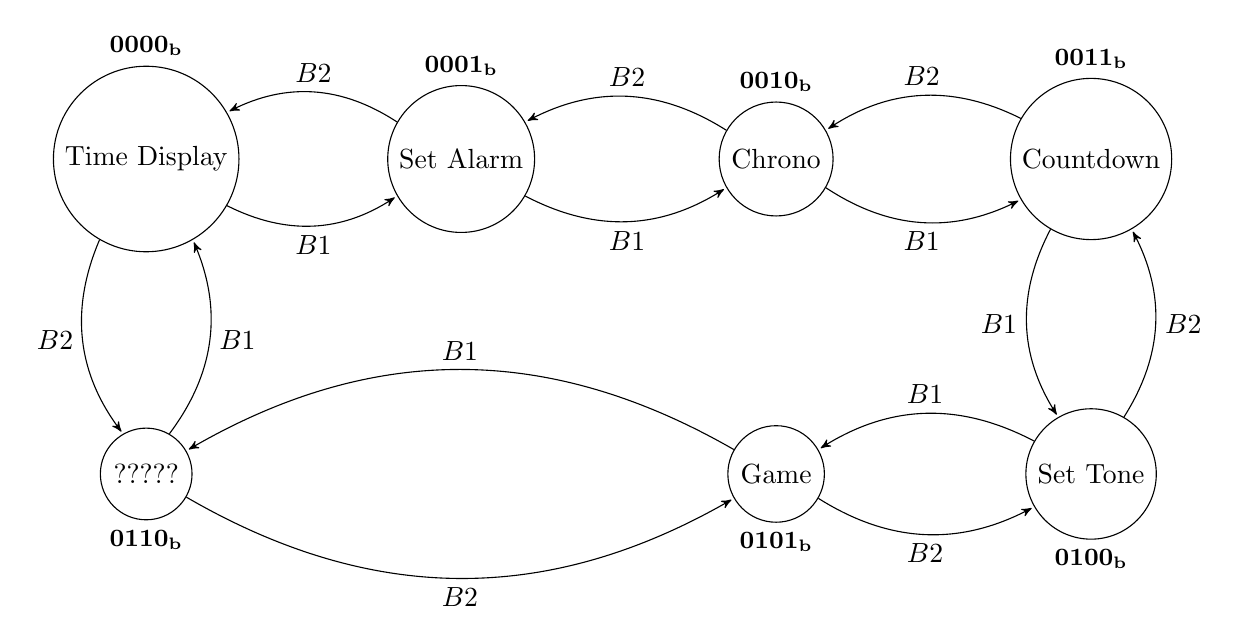
\begin{tikzpicture}[->,>=stealth',shorten >=1pt,auto,node distance=4cm,
        scale = 1,transform shape]

  \node[state][label={\small\textbf{0000\textsubscript{b}}}] (Time Display) [] {Time Display};
  \node[state][label={\small\textbf{0001\textsubscript{b}}}] (Set Alarm) [right of=Time Display] {Set Alarm};
  \node[state][label={\small\textbf{0010\textsubscript{b}}}] (Chronometer) [right of=Set Alarm] {Chrono};
  \node[state][label={\small\textbf{0011\textsubscript{b}}}] (Countdown) [right of=Chronometer] {Countdown};
  \node[state][label=below:{\small\textbf{0100\textsubscript{b}}}] (Set Tone) [below of=Countdown] {Set Tone};
  \node[state][label=below:{\small\textbf{0101\textsubscript{b}}}] (Game) [left of=Set Tone] {Game};
  \node[state][label=below:{\small\textbf{0110\textsubscript{b}}}] (NA) [below of=Time Display] {?????};

  \path (Time Display) edge [bend right]           node[below] {$B1$} (Set Alarm)
        (Set Alarm) edge [bend right]              node[below] {$B1$} (Chronometer)
        (Chronometer) edge[bend right]              node[below] {$B1$} (Countdown)
        (Countdown) edge[bend right]            node[left] {$B1$} (Set Tone)
        (Set Tone) edge [bend right]            node[above] {$B1$} (Game)
        (Game) edge  [bend right]             node[above] {$B1$} (NA)
        (NA) edge [bend right]               node[right] {$B1$} (Time Display)
        
        
  		(Time Display) edge[bend right]              node[left] {$B2$} (NA)
        (NA) edge[bend right]              node[below] {$B2$} (Game)
        (Game) edge[bend right]              node[below] {$B2$} (Set Tone)
        (Set Tone) edge[bend right]              node[right] {$B2$} (Countdown)
        (Countdown) edge[bend right]              node[above] {$B2$} (Chronometer)
        (Chronometer) edge[bend right]              node[above] {$B2$} (Set Alarm)
        (Set Alarm) edge[bend right]              node [above]{$B2$} (Time Display);
\end{tikzpicture}
\end{center}
\subsection{Machines d'états finis secondaires}
(Spécialement intéressantes incluant solution à l'utilisation de la carte périphérique)
\subsection{Solutions techniques aux problèmes de développement}
(avec screens de logisim)
\end{document}